%\documentclass[preprint]{aastex}
\documentclass[onecolumn]{emulateapj}
\usepackage{url}
\usepackage{multirow}
\usepackage{amsmath}
\usepackage{xcolor}
\usepackage{enumerate}
\usepackage{listings}
\lstset{language=Python,numbers=left,numberstyle=\tiny ,stepnumber=1,numbersep=8pt,basicstyle=\footnotesize, breaklines=true}
%\citestyle{aa} 
\usepackage{affils}
%\bibliographystyl{apj_w_etal}

\newcommand{\etal}{{et al.\/}}
\newcommand{\Prob}{\mathtt{P}}
\newcommand{\logL}{\log\mathcal{L}}
\newcommand{\unit}[1]{\footnotesize #1}
\newcommand{\PAPER}{\mathrm{PAPER}}
\newcommand{\hMpci}{h\ {\rm Mpc}^{-1}}

%%define graphics path to search for images
%\graphicspath{{./data/}}

\newcommand{\Nconf}{31}
\newcommand{\Nsrc}{32}
\definecolor{orange}{RGB}{255,127,0}

\tabletypesize{\scriptsize}

	% End definitions

%\slugcomment{DRAFT: \today}

\begin{document}
\title{The Effect of Fringe Rate Filter Shape on the Power Spectrum}
\shortauthors{Kolopanis}


\DeclareAffil{asu}{Department of Physics, Arizona State University, Tempe, Arizona 85203}
\DeclareAffil{sese}{School of Earth and Space Exploration, Arizona State University, Tempe, Arizona 85203}


\affilauthorlist{
  Matthew Kolopanis%\affils{asu,sese}
  }

\maketitle
This memo outlines the changes to the PAPER-64 power spectrum pipeline after Ali et al 2015. The application of the fringe rate filter is the final step in the PAPER analysis pipeline. The filter sets the total effective integration time and number of independent sky samples in the lst-binned. Fringe rate filtering also suppresses "non-sky" systematic modes. Small changes to the shape of the filter can have a fairly dramatic impact the power spectrum.

The fringe rate filter used in Ali 2015 (A15 hereafter) report on the PSA64 power spectrum is notably different from that described in Parsons et al Beam sculpting and fringe rate filter paper. This memo steps through the differences between the two to reconstruct the shape of the A15 filter and assess the impact on the data.

First, we compute the power spectrum of the data used to make the A15 power spectrum. Next we reconstruct the filter applied to the data and get a power spectrum which is close to the A15 result. Finally, we apply the "optimal" filter and get a power spectrum. All results ahve been corrected for signal loss using the method in A15.

\section{Power Spectrum of A15}{

We use the data from the A15 as input to the power spectrum pipeline to ensure the local version of the pipeline is in agreement with the A15 results.

Figure \ref{fig:compare_apj} displays the A15 power spectrum, to a spectrum made with the fringe-rate filtered data used by A15. The spectra show good agreement in the range $.15< k< .5 \hMpci $, as such it is reasonable to assume the power spectrum pipeline is working properly on enterprise at ASU.


\begin{figure}[h]
\centering
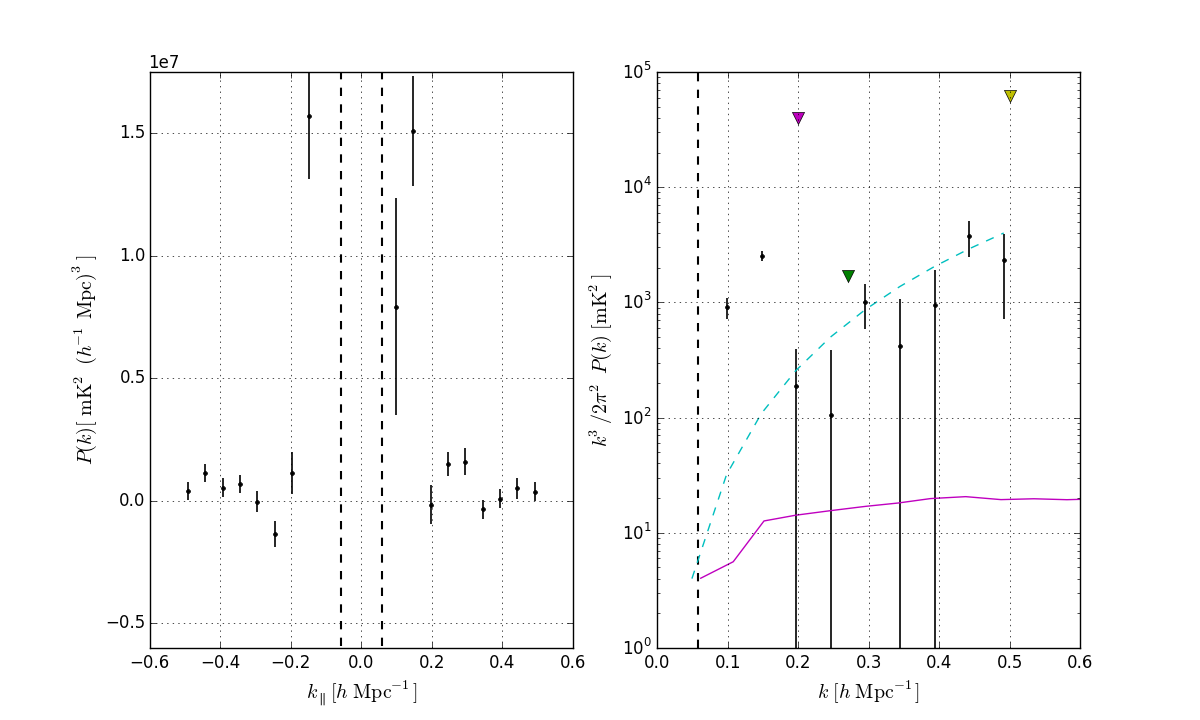
\includegraphics[width=.6\textwidth]{data/ali_et_al_pspec.png}

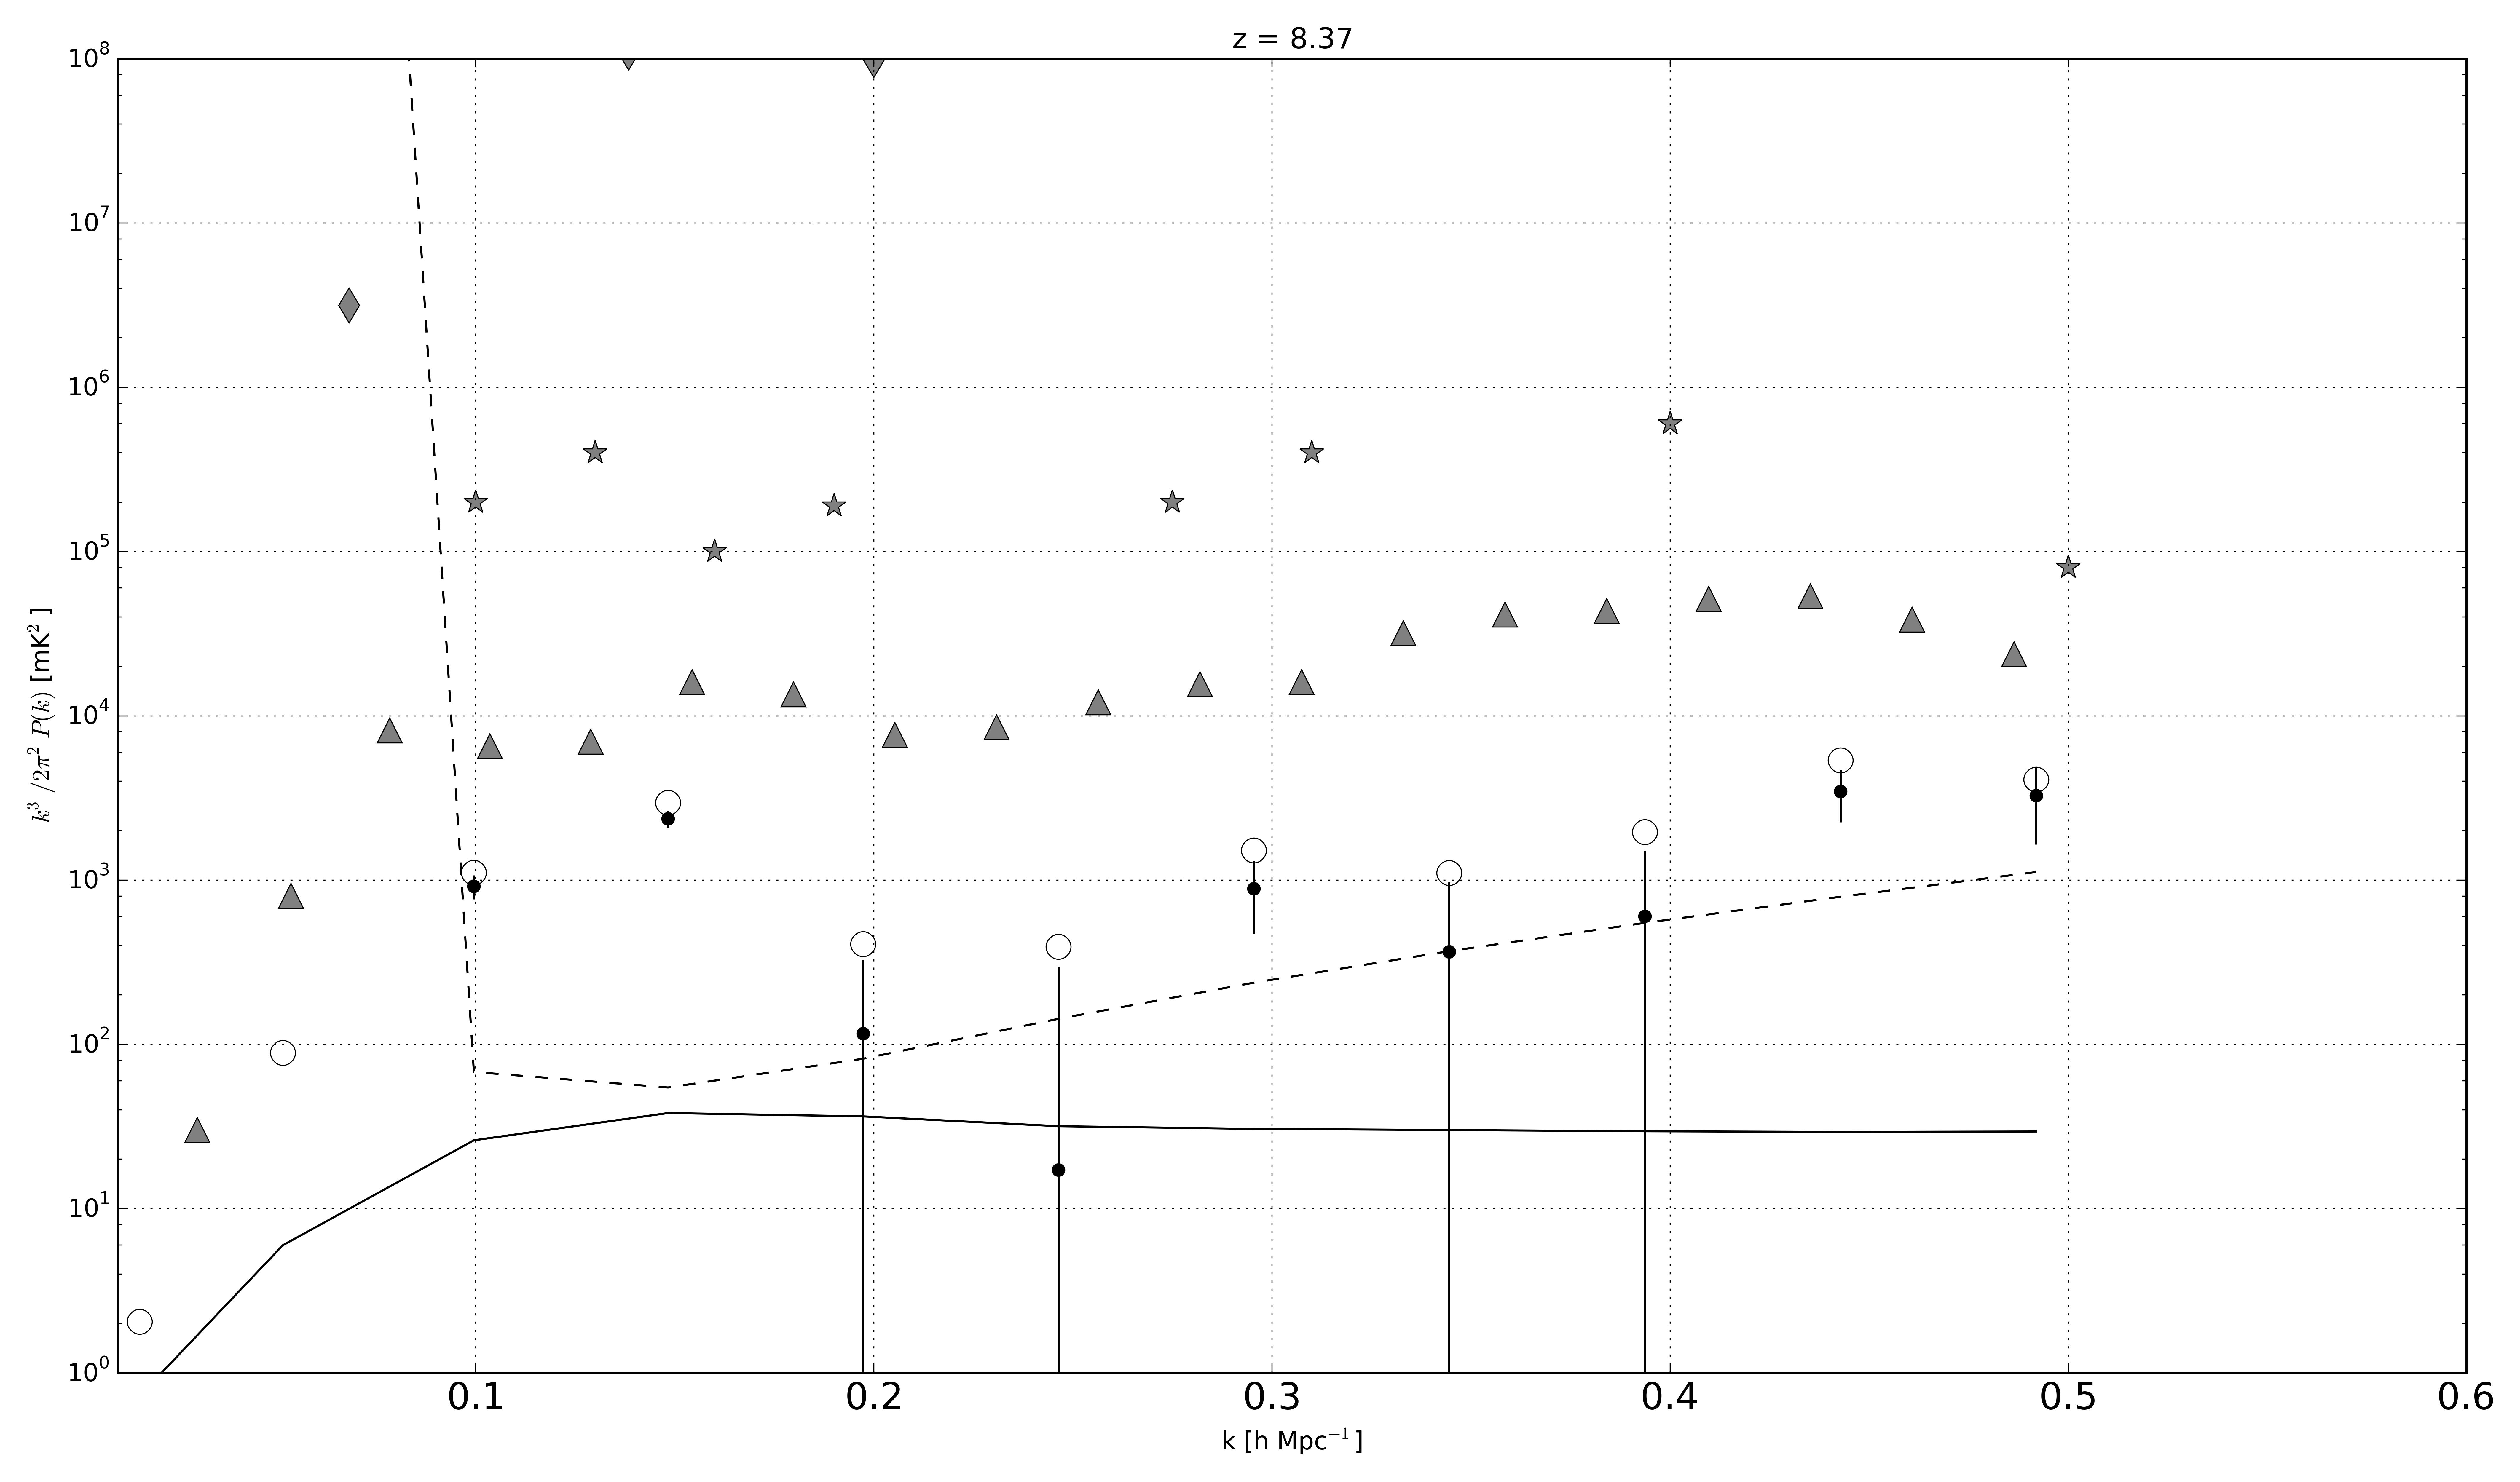
\includegraphics[width=.5\textwidth]{data/pspec_Mar14_vanilla_ali_apj_frf_95_115_I_comparison.png}
\caption{\label{fig:compare_apj} Top: the apj v002 power spectrum from Ali et al 2015. Bottom: Open circles are 2$\sigma$ A15 published data points (same as plotted in top figure). Black dtos are our run of the power spectrum code on archived lst-binned frf filtered data used in the A15 paper. The only difference is a slightly higher signal loss which accounts for the offset. All error bars are 2 sigma}
\end{figure}
}

\section{Reconstructing the A15 Filter}{
The following steps were taken to try to recreate the A15 frf:

\begin{enumerate}
\item capo/src/frf\_conv.py  mk\_fng(bl, eq)
\begin{enumerate}
\item this is the mk\_fng for the optimal frf
\end{enumerate} 

\item capo/src/frf\_conv.py  mk\_fng\_alietal(bl,eq)
\begin{enumerate}
\item This is the mk\_fng used in A15
\end{enumerate}

frf\_conv.py should look like:
\begin{lstlisting}[firstnumber=24,name=frf_conv.py,fontadjust]
def mk_fng(bl, eq):
     '''Return fringe rates given eq coords and a baseline vector (measured in wavelengths) in eq coords'''
   return -2*n.pi/a.const.sidereal_day * n.dot(n.cross(n.array([0,0,1.]),bl), eq)
  
fringe used in ali et.al to degrade optimal fringe rate filter.
def mk_fng_alietal(bl, eq):
    '''Return distorted fringe rates for given eq coordinates and a baseline vector (measured in wavelengths) in eq coords. This was the version used in ali et.al'''
    ey, ex, ez = eq#yes, ex and ey are flipped.
    return 2*n.pi/a.const.sidereal_day * (bl[0]*ex + bl[1]*ey * n.sqrt(1-ez**2))
\end{lstlisting}

\item capo/mjk/scripts/frf\_filter.py \footnote{
While it is not necessary to use this python script to apply a fringe rate filter to data, I used this script in accompaniment with capo/mjk/scripts/batch\_frf\_filter.sh to filter all data contained in a directory whose sub-directories are named "even" and "odd"  with the A15 reconstruction filter (e.g. lstbin\_psa64\_no\_frf/{even,odd}/sep0,1 ..etc). This script would be executed in lstbin\_psa64\_no\_frf/}

\begin{enumerate}
\item this script applies the frf selected by the user on data passed as arguments
\item command line options allow for the application of the optimal or ali et al frf 
\item can fine tune the frf by setting channel, maxfr, baseline length scaling factor, alietal flag
\item setting the following parameters for the ali et. al filter
\begin{enumerate}
\item chan=160
\item --alietal
\end{enumerate}
\end{enumerate}
\end{enumerate}

\begin{figure}[t]
\centering
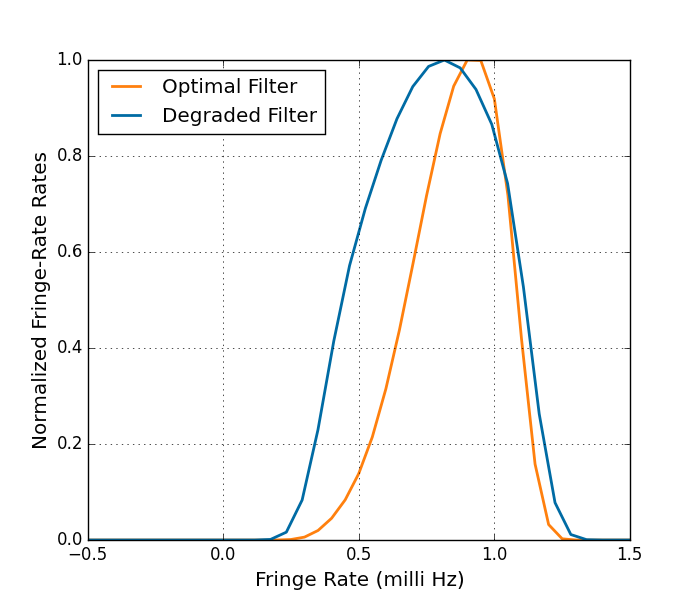
\includegraphics[width=.4\textwidth]{data/alietal_frf.png}
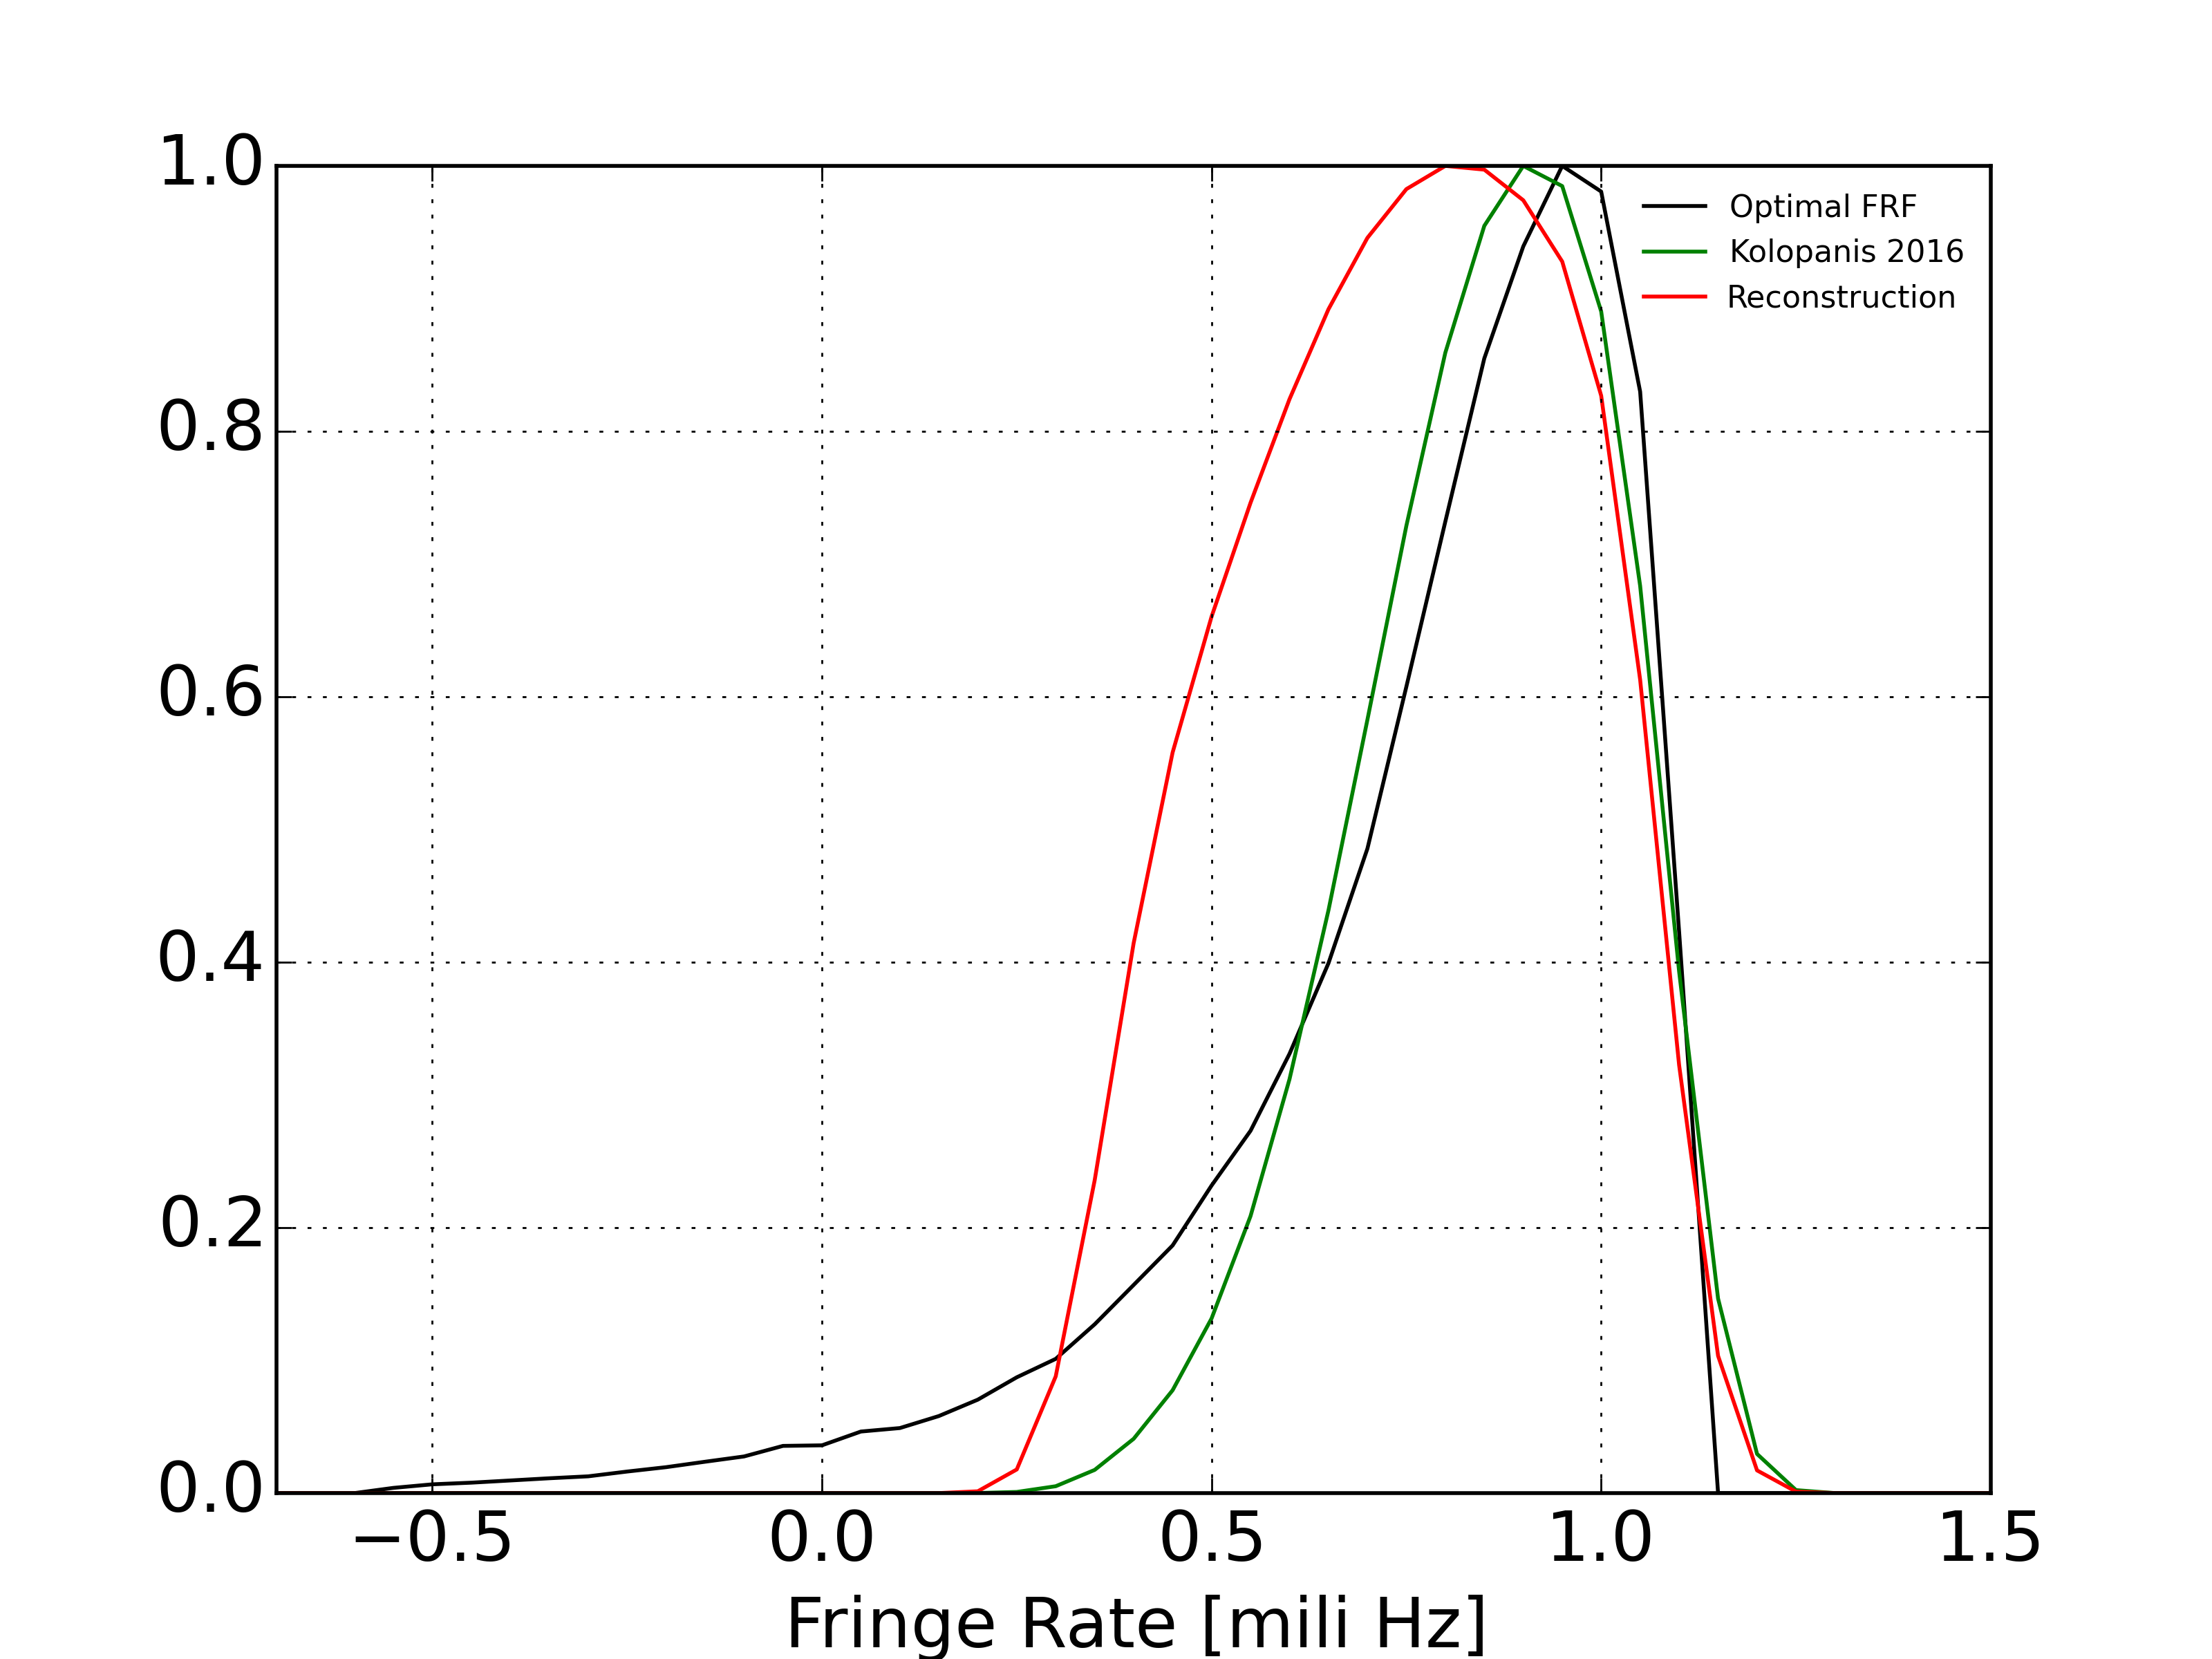
\includegraphics[width=.45\textwidth]{data/frf_comparison.png}
\caption{\label{fig:frf} Left: the A15 fringe rate filter. Right: the optimal frf, K16 frf, and the A15 reconstruction \vspace{.35cm}}
\end{figure} 

Note use of channel 160 to create the sky fringe as per Zaki's instructions. In A15, this fringe is used to make a fringe rate profile, this profile is then interpolated between frequency bins. 


A comparison of the A15 filter, the optimal filter, the K16 filter and the A15 reconstruction filter are shown in Figure \ref{fig:frf}. %While the shapes of the A15 and reconstruction filter are similar, some differences are still apparent.




\begin{figure}[tb]
\centering
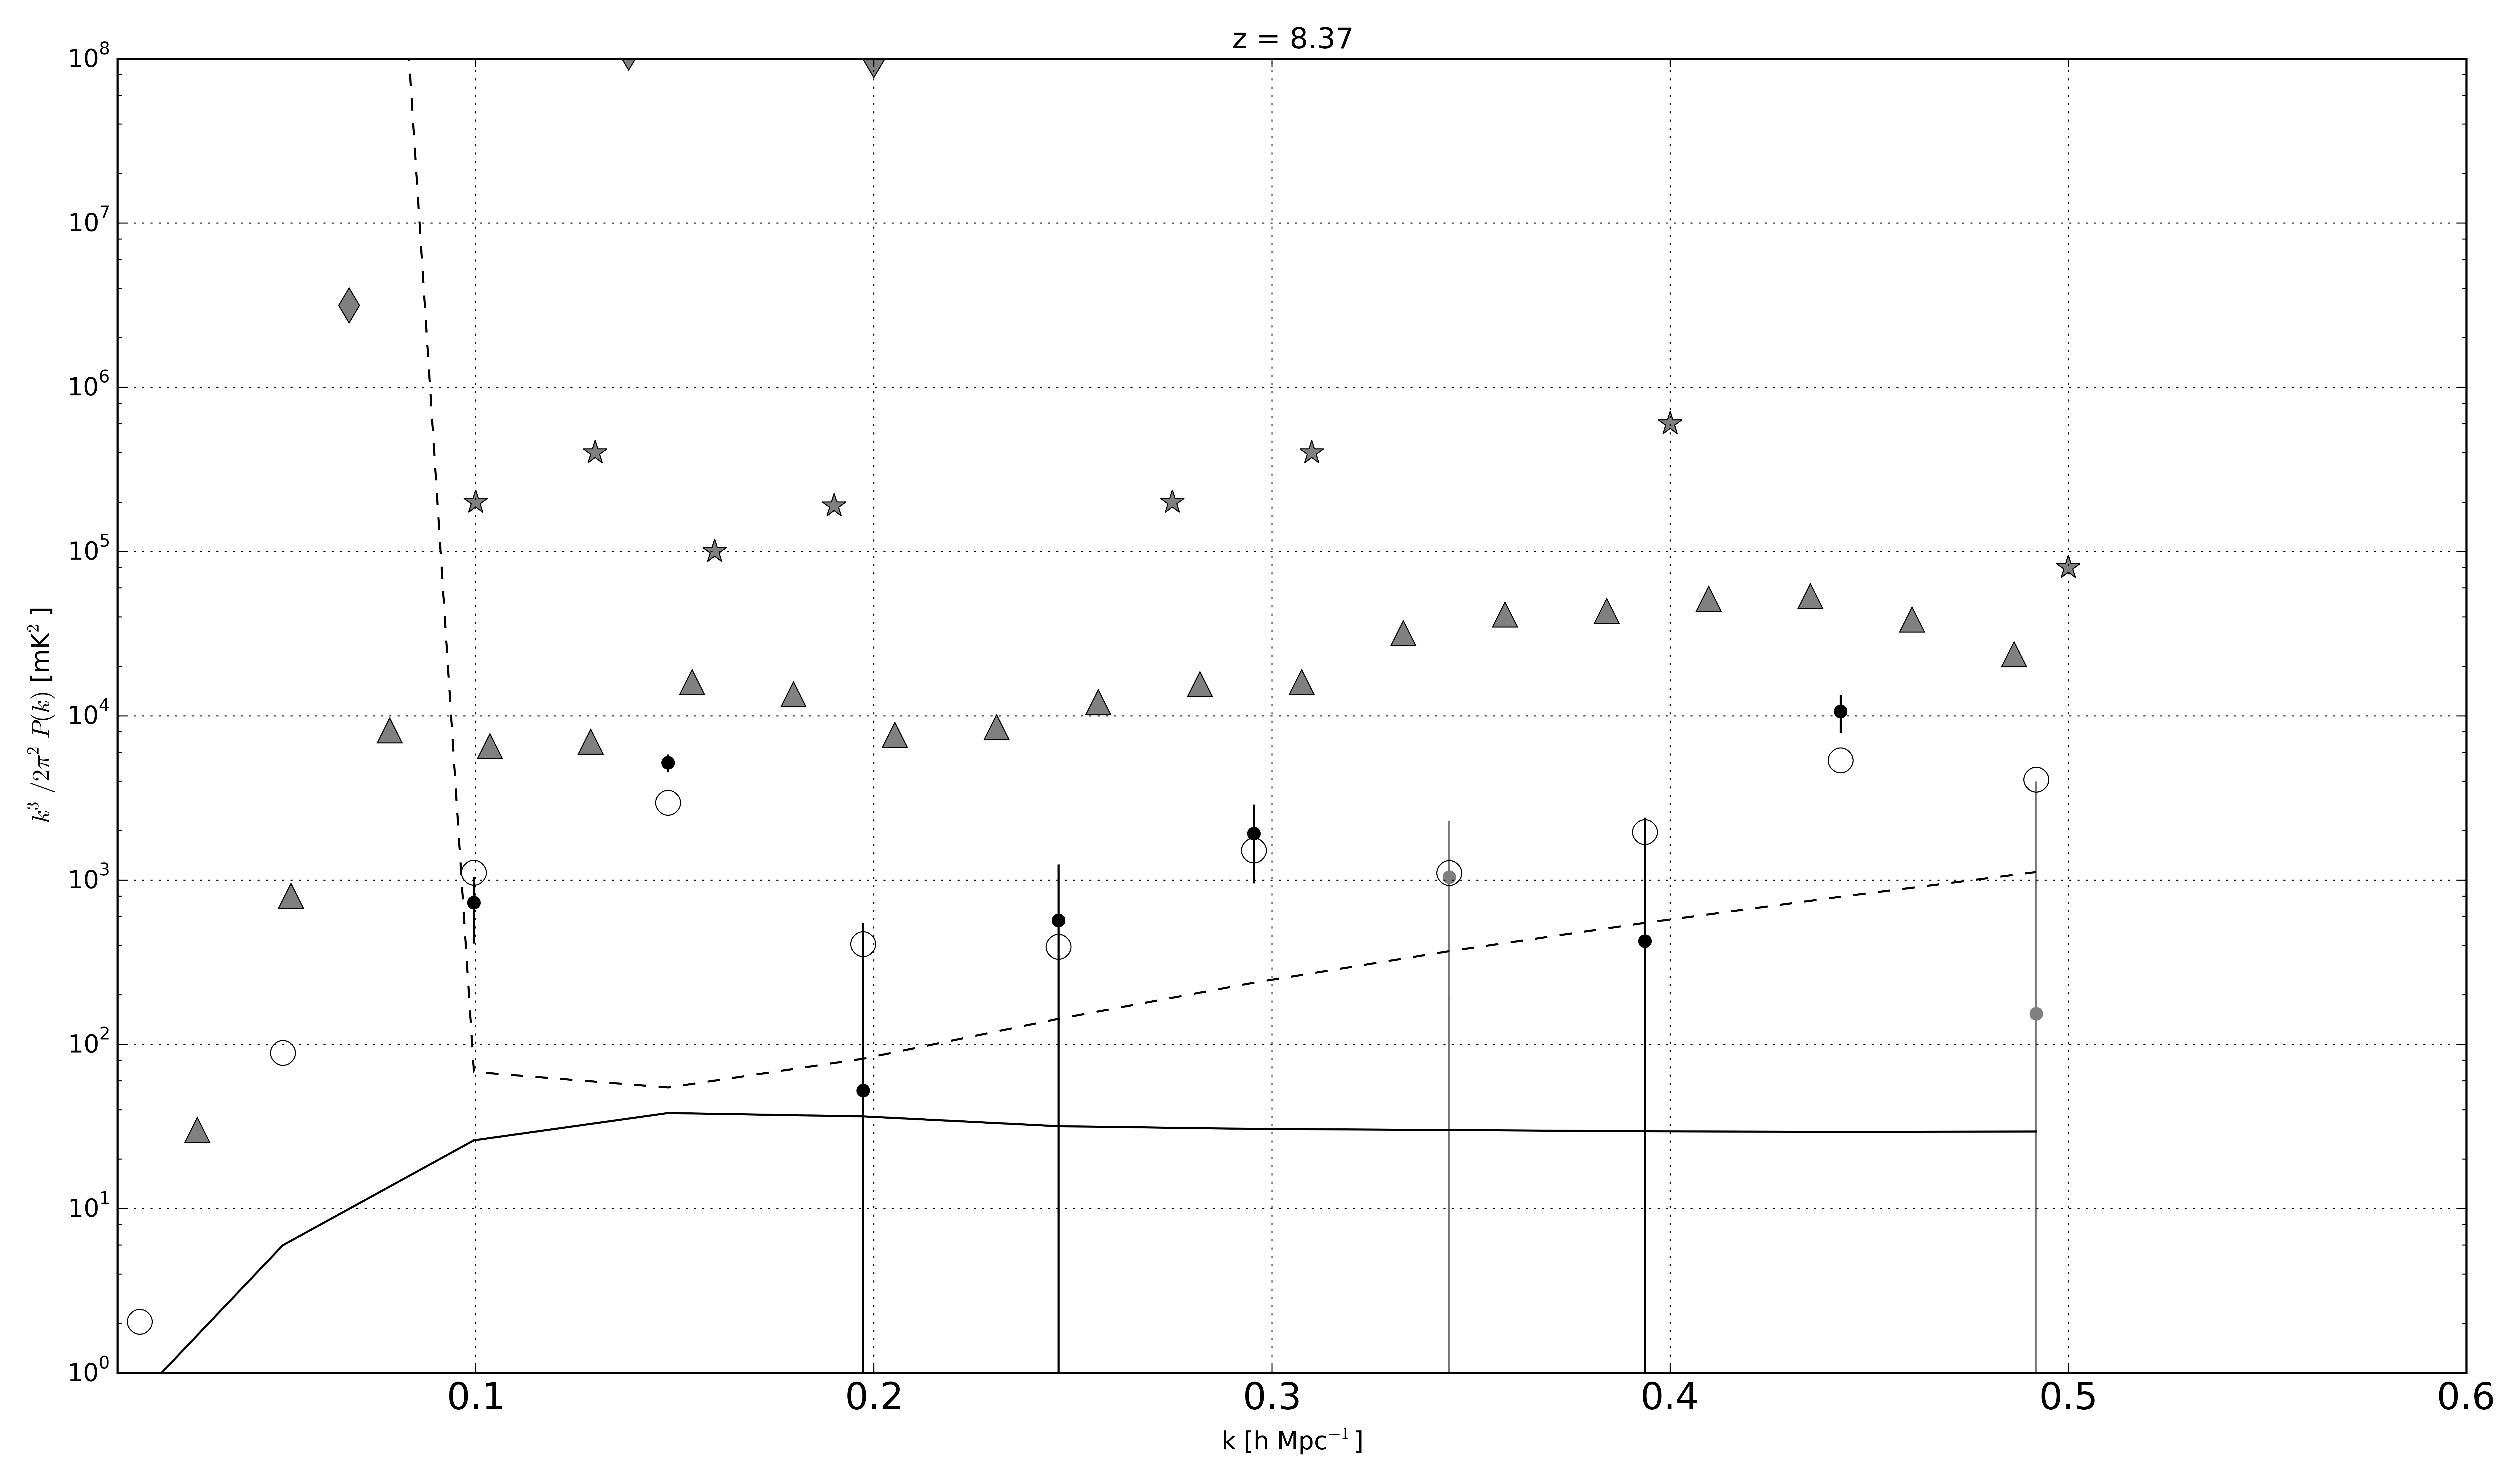
\includegraphics[width=.8\textwidth]{data/pspec_Mar17_vanilla_ali_frf_recon_95_115_I_comparison.png}
\caption{\label{fig:recon_apj}Black dots with error bars show the power spectrum after applying the reconstructed A15 frf. Open circles in the lower image indicate 2$\sigma$ upper bounds from the A15.}
\end{figure}
The reconstruction filter is then applied to the data, the resulting power spectrum is shown in Figure \ref{fig:recon_apj}.

}

\section{Optimal Fringe Rate Filter}{
To construct the optimal fringe rate filter used in the following alterations should be made:

\begin{enumerate}

\item capo/mjk/scripts/frf\_filter.py
\begin{enumerate}
\item do not set the alietal flag
\item use chan 101 or 105
\end{enumerate}
\end{enumerate}
\begin{figure}[tb]
\centering
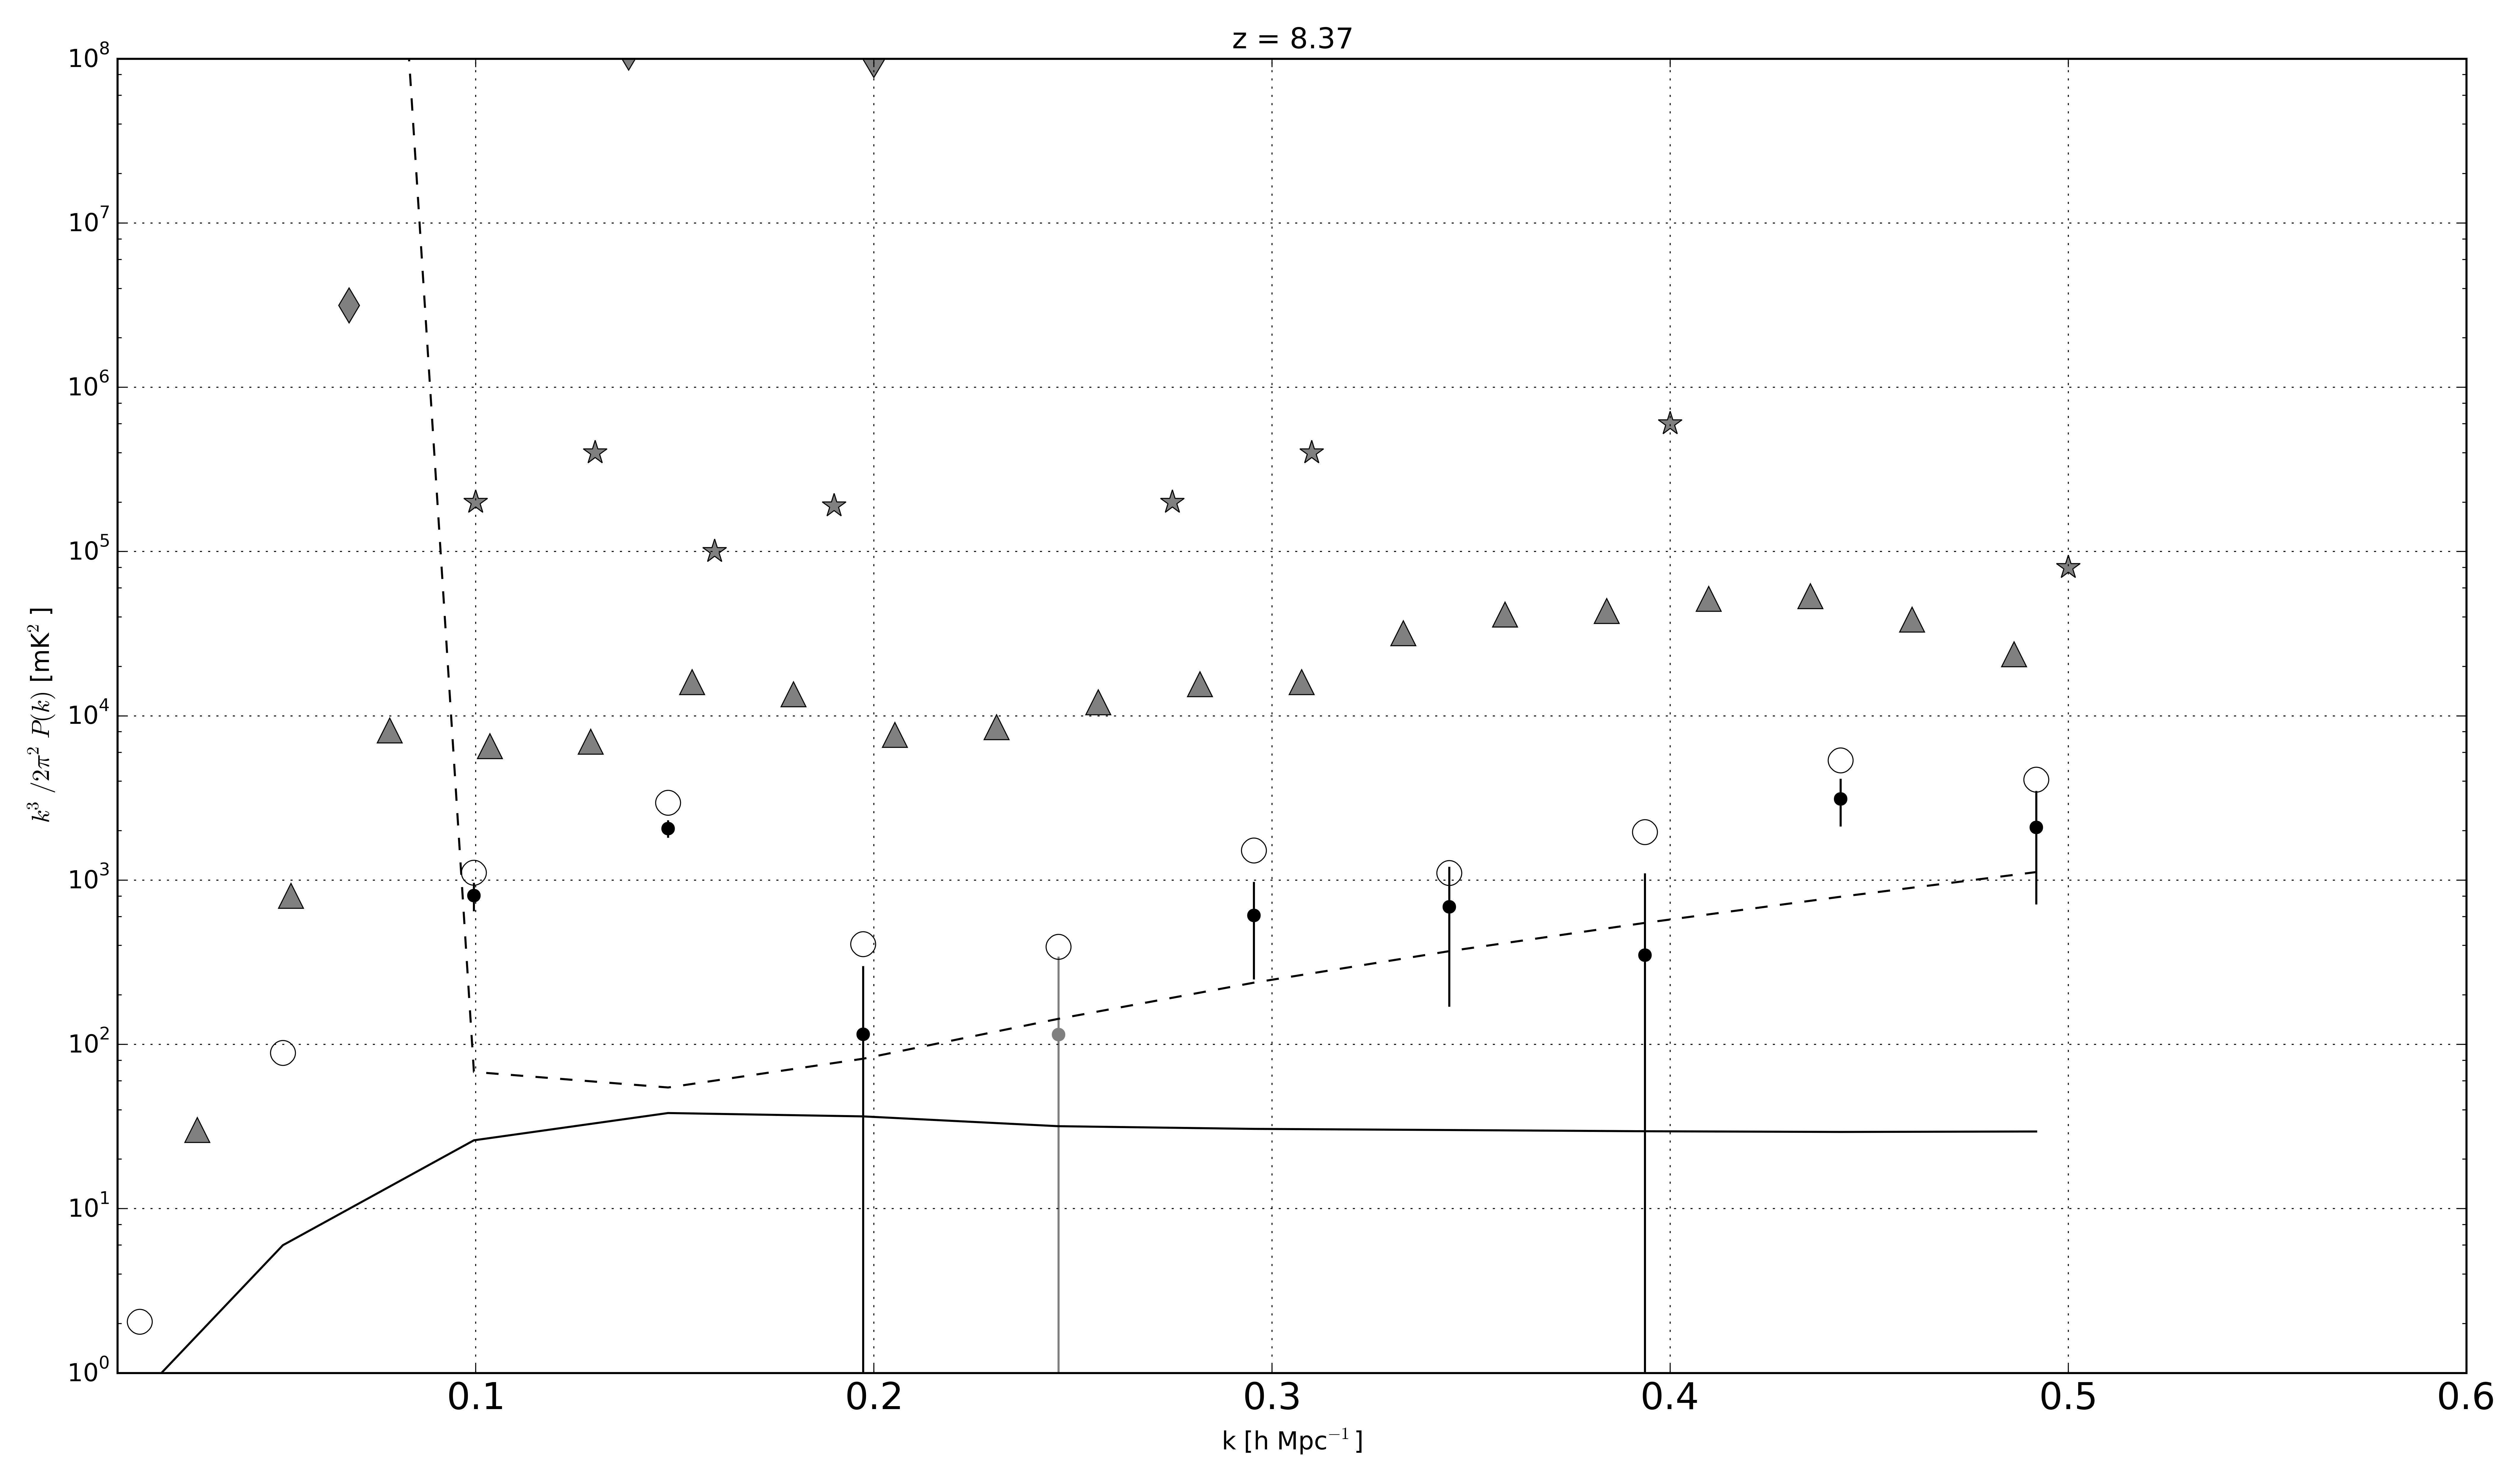
\includegraphics[width=.8\textwidth]{data/psa64_ali_reconstruction.png}
\caption{\label{fig:optimal_pspec} Black dots with error bars show the power spectrum after applying the optimal filter. Open circles in the lower image indicate 2$\sigma$ upper bounds from the A15.}
\end{figure}

Any script can be used to filter unfiltered data. I use capo/mjk/scripts/batch\_frf\_filter.sh which again should be executed in a directory like lstbin\_psa64\_nofrf/ whose sub-directories are "even" and "odd".

A power spectrum from date filtered with the optimal fringe rate filter is shown in Figure \ref{fig:optimal_pspec}.
}


\end{document}